\documentclass[a4paper,11pt]{article}
\usepackage[T1]{fontenc}
\usepackage[utf8]{inputenc}
\usepackage{lmodern}
\usepackage{microtype}
\usepackage[a4paper,margin=1in,headheight=15pt,headsep=14pt]{geometry}
\usepackage{amsmath,amssymb}
\usepackage{graphicx}
\usepackage{booktabs}
\usepackage{adjustbox}
\usepackage[table,svgnames]{xcolor}
\usepackage[most]{tcolorbox}
\tcbuselibrary{skins,breakable}
\usepackage{tikz}
\usepackage{pifont}
\newcommand{\glyphHand}{\ding{43}}
\newcommand{\glyphPencil}{\ding{46}}
\usepackage{enumitem}
\setlist{leftmargin=1.5em,topsep=4pt,itemsep=3pt}
\newlist{steps}{enumerate}{1}
\setlist[steps]{label=\textbf{Step \arabic*.},
  leftmargin=4.4em, labelwidth=3.8em, labelsep=0.6em, labelindent=0pt,
  align=left, topsep=5pt, itemsep=6pt}
\usepackage{parskip}
\usepackage{fancyhdr}
\usepackage{titlesec}
\usepackage[hidelinks]{hyperref}
\usepackage{xurl}
\hypersetup{breaklinks=true}
\definecolor{navy}{HTML}{21355E}\definecolor{navyrule}{HTML}{21355E}
\definecolor{inktext}{HTML}{1A202C}\definecolor{mutedtext}{HTML}{6B7280}
\definecolor{intuFrame}{HTML}{2C5AA0}\definecolor{intuFill}{HTML}{F4F7FC}
\definecolor{everyFrame}{HTML}{8A5A1E}\definecolor{everyFill}{HTML}{FBF1E3}
\definecolor{workFrame}{HTML}{2E7D52}\definecolor{workFill}{HTML}{F1F8F3}
\definecolor{watchFrame}{HTML}{B23A48}\definecolor{watchFill}{HTML}{FBF1F2}
\definecolor{keyFrame}{HTML}{6A4C93}\definecolor{keyFill}{HTML}{F4F0F9}
\color{inktext}\hypersetup{linkcolor=navy,urlcolor=navy,citecolor=navy}
\tcbset{housecallout/.style 2 args={enhanced,breakable,colback=#2,colframe=#1,boxrule=0.6pt,arc=2.4pt,outer arc=2.4pt,left=10pt,right=10pt,top=9pt,bottom=9pt,before skip=11pt,after skip=11pt,fontupper=\normalsize,coltitle=white,fonttitle=\bfseries\sffamily\small,attach boxed title to top left={xshift=6mm,yshift=-3mm},boxed title style={colback=#1,colframe=#1,rounded corners,arc=3pt,boxrule=0pt,left=6pt,right=6pt,top=2pt,bottom=2pt}}}
\newtcolorbox{intuition}{housecallout={intuFrame}{intuFill},title={\raisebox{-0.05ex}{\glyphHand}\,\ The intuition}}
\newtcolorbox{everyday}{housecallout={everyFrame}{everyFill},title={\raisebox{-0.05ex}{$\bigstar$}\,\ Everyday picture}}
\newtcolorbox{worked}[1]{housecallout={workFrame}{workFill},title={\raisebox{-0.05ex}{\glyphPencil}\,\ Worked example: #1}}
\newtcolorbox{watchout}{housecallout={watchFrame}{watchFill},title={\raisebox{-0.05ex}{\ding{55}}\,\ Watch out}}
\newtcolorbox{keytake}{housecallout={keyFrame}{keyFill},title={\raisebox{-0.05ex}{\ding{51}}\,\ Key takeaway}}
\newcommand{\CourseShort}{SEML Companion}\newcommand{\SessionNo}{1}\newcommand{\LectureTitle}{Foundations of ML Systems Engineering}
\pagestyle{fancy}\fancyhf{}
\fancyhead[L]{\footnotesize\color{mutedtext}\textsf{\CourseShort}}
\fancyhead[R]{\footnotesize\color{mutedtext}\textsf{Session \SessionNo\ \textperiodcentered\ \LectureTitle}}
\fancyfoot[C]{\footnotesize\color{mutedtext}\thepage}
\renewcommand{\headrulewidth}{0.4pt}\renewcommand{\footrulewidth}{0pt}
\renewcommand{\headrule}{\hbox to\headwidth{\color{navyrule!55}\leaders\hrule height \headrulewidth\hfill}}
\titleformat{\section}{\sffamily\Large\bfseries\color{navy}}{\thesection}{0.8em}{}[{\vspace{2pt}\color{navy!70}\titlerule[0.8pt]}]
\titleformat{\subsection}{\sffamily\large\bfseries\color{navy!92}}{\thesubsection}{0.7em}{}
\titlespacing*{\section}{0pt}{16pt}{8pt}\titlespacing*{\subsection}{0pt}{12pt}{4pt}
\newcommand{\titlebanner}[4]{\begin{tcolorbox}[enhanced,breakable=false,colback=navy,colframe=navy,boxrule=0pt,arc=3pt,outer arc=3pt,left=16pt,right=16pt,top=16pt,bottom=16pt,before skip=2pt,after skip=14pt,width=\linewidth]{\sffamily\footnotesize\bfseries\color{white!85}\MakeUppercase{#1}}\par\vspace{6pt}{\sffamily\bfseries\fontsize{30}{34}\selectfont\color{white}#2\par}\vspace{5pt}{\sffamily\large\color{white!88}#3\par}\vspace{9pt}{\color{white!55}\rule{\linewidth}{0.4pt}}\par\vspace{6pt}{\sffamily\footnotesize\color{white!82}#4\par}\end{tcolorbox}}
\newcommand{\vocab}[1]{\textbf{\color{navy}#1}}
\newcommand{\housefig}[2]{%
  \begin{figure}[htbp]
    \centering
    \includegraphics[width=\linewidth]{#1}%
    \caption{#2}
  \end{figure}%
}
\begin{document}
\thispagestyle{fancy}
\titlebanner{AIMLCZG546 \textperiodcentered\ Session 1 \textperiodcentered\ Companion Reader}{Foundations of ML Systems Engineering}{SDLC, Data Science, ML Pipeline, Three Generations, Domains and LLMs}{Session 1 \textperiodcentered\ Read alongside the lecture slides \textperiodcentered\ Every concept explained from scratch}

\noindent\textbf{How to use this companion.} Five colour-coded boxes appear throughout. \textcolor{intuFrame}{\textbf{Blue}} boxes give the core intuition in plain words. \textcolor{everyFrame}{\textbf{Amber}} boxes anchor the idea to an everyday situation you already understand. \textcolor{workFrame}{\textbf{Green}} boxes walk through a concrete example step by step. \textcolor{watchFrame}{\textbf{Red}} boxes flag common pitfalls. \textcolor{keyFrame}{\textbf{Purple}} boxes state the single most important line to remember.

%==============================================================
\section{Software Development Life Cycle (SDLC)}
%==============================================================

Every software product you use was built using a repeatable process. Think of a banking app, a ride-hailing service, or a hospital record system. That process is the \vocab{Software Development Life Cycle (SDLC)}. It is a structured sequence of phases. It guides a team from an idea to a shipped product. Then it keeps that product running.

\begin{intuition}
The SDLC is a recipe. A recipe tells a chef what to do, in what order, and when each step is done. The SDLC does the same for a software team. First, understand what to build. Then design it. Then write the code. Then test it. Then ship it. Then maintain it.
\end{intuition}

\begin{everyday}
Think of building a house. Before a single brick is laid, the owner explains their needs (requirements). An architect draws blueprints (design). Builders construct the walls (implementation). Inspectors check for cracks (testing). The family moves in (deployment). A plumber fixes leaks over the years (maintenance). A software team follows the same six steps in the same order.
\end{everyday}

The six classic SDLC phases are:
\begin{enumerate}
  \item \textbf{Planning} — what are we building, and is it feasible?
  \item \textbf{Requirements Analysis} — what exactly must the system do?
  \item \textbf{System Design} — how will it be structured (architecture, database, APIs)?
  \item \textbf{Implementation (Coding)} — write the actual code.
  \item \textbf{Testing \& Quality Assurance} — does it work correctly and safely?
  \item \textbf{Deployment \& Maintenance} — release it and keep it healthy.
\end{enumerate}

\subsection{Roles in a Software Team}

A software project involves many specialists, each responsible for a different slice of the process.

\begin{center}
\resizebox{\linewidth}{!}{%
\begin{tabular}{lll}
\toprule
\textbf{Role} & \textbf{Phase focus} & \textbf{Core responsibility} \\
\midrule
Business Analyst & Requirements & Translates business needs into technical specifications \\
Project Manager & All phases & Plans timelines, manages risks, tracks progress \\
Product Owner & Requirements + Delivery & Represents users; prioritises features \\
Software Architect & Design & Designs high-level structure and technology choices \\
UX/UI Designer & Design + Testing & Creates user interfaces and experience flows \\
Developer & Implementation & Writes and reviews code \\
QA / Tester & Testing & Writes and runs tests; reports defects \\
Scrum Master & All (in Agile) & Removes blockers; facilitates Agile ceremonies \\
Team Lead & Implementation & Guides the developer team; does code review \\
\bottomrule
\end{tabular}}
\end{center}

\begin{worked}{Who does what on a food-delivery app}
Imagine building a Swiggy-like app. Each role owns a slice of the work.
\begin{steps}
  \item \textbf{Business Analyst.} Interviews restaurant owners and customers. Writes a requirements document.
  \item \textbf{Software Architect.} Decides to use microservices: separate services for orders, payments, and delivery.
  \item \textbf{UX Designer.} Draws the app screens and the user flow.
  \item \textbf{Developers.} Build each service and write the code.
  \item \textbf{QA Engineers.} Test that an order deducts the right amount and notifies the right partner.
  \item \textbf{Project Manager.} Ensures the first release ships before the next festive season.
  \item \textbf{DevOps Engineer.} Deploys the app to the cloud and sets up monitoring.
\end{steps}
\end{worked}

\subsection{Evolution to Cloud-Native}

Traditional SDLC produced software released once every six to twelve months. Modern software teams ship multiple times per day. The shift happened through three combined innovations:
\begin{itemize}
  \item \vocab{Agile} --- work in short sprints (1--3 weeks); deliver working software continuously.
  \item \vocab{DevOps} --- development and operations teams share responsibility. Testing and deployment are automated.
  \item \vocab{Cloud Native} --- use containers (Docker), orchestration (Kubernetes), and microservices. Systems become small, independent, and always running.
\end{itemize}

\housefig{figures/figsdlcflow.png}{The six SDLC phases in order. Each phase feeds the next. Read from left to right.}

\noindent\textbf{Where this shows up in ML/AI.} Every ML team runs inside some form of SDLC. ML adds new phases: data collection, model training, and evaluation. These do not appear in traditional SDLC. This course shows how to adapt the SDLC to handle them.

\begin{keytake}
The SDLC is the backbone of every software project. It doesn't change when ML enters the picture --- ML adds new phases inside it.
\end{keytake}

%==============================================================
\section{Data Science and the AI/ML Landscape}
%==============================================================

\vocab{Data Science} is the study of data: collecting it, cleaning it, analysing it, and drawing actionable insights from it. The goal is to extract value that would otherwise remain hidden inside raw numbers.

\begin{intuition}
Imagine a mountain of sand. Data Science is the sieve that separates the gold flakes (insights) from the rest (noise). The sieve has five layers: collect the sand, clean it, analyse it, build a prediction model, then show the results.
\end{intuition}

\begin{everyday}
A doctor reviews thousands of patient records. They notice: ``patients with these three symptoms are 80\,\% more likely to develop diabetes.'' That is data science. They collected data (records), cleaned it (removed duplicates), and spotted the pattern. They built a mental prediction model. Then they shared the finding --- the 80\,\% figure --- with colleagues.
\end{everyday}

The standard Data Science workflow:
\begin{enumerate}
  \item \textbf{Data Collection} — gather raw data from databases, APIs, sensors, surveys.
  \item \textbf{Data Preprocessing} — fix missing values, remove duplicates, normalise formats.
  \item \textbf{Exploratory Data Analysis (EDA)} — visualise distributions, spot correlations, understand the data.
  \item \textbf{Modelling} — train a statistical or ML model on the cleaned data.
  \item \textbf{Deployment \& Visualisation} — share the predictions or dashboards with decision-makers.
\end{enumerate}

\subsection{Where AI, ML, and Data Science Overlap}

These three terms are often confused. Here is the precise relationship:

\begin{center}
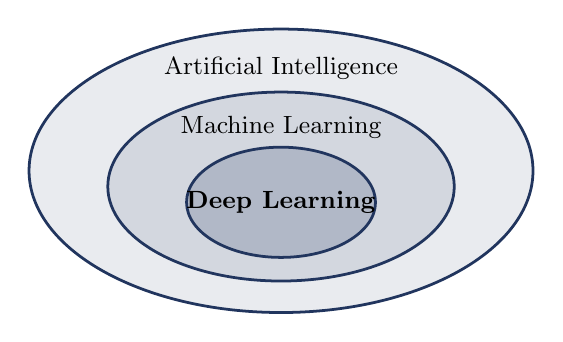
\begin{tikzpicture}[font=\small]
  \draw[fill=navy!10,draw=navy,line width=1pt] (0,0) ellipse (3.2cm and 1.8cm);
  \draw[fill=navy!20,draw=navy,line width=1pt] (0,-0.2) ellipse (2.2cm and 1.2cm);
  \draw[fill=navy!35,draw=navy,line width=1pt] (0,-0.4) ellipse (1.2cm and 0.7cm);
  \node at (0,-0.4) {\textbf{Deep Learning}};
  \node at (0,0.55) {Machine Learning};
  \node at (0,1.3) {Artificial Intelligence};
\end{tikzpicture}
\end{center}

\begin{itemize}
  \item \vocab{Artificial Intelligence (AI)} — the broad goal of making machines behave intelligently.
  \item \vocab{Machine Learning (ML)} — a subset of AI where machines learn from data rather than being hand-programmed with rules.
  \item \vocab{Deep Learning} — a subset of ML that uses multi-layer neural networks; excels when data is large and unstructured (images, text, audio).
  \item \vocab{Data Science} — overlaps all three; focuses on extracting insights from data, often using ML as a tool.
\end{itemize}

\noindent\textbf{Where this shows up in ML/AI.} Data Science is often the starting point of an ML project. Before a model can be trained, a data scientist must collect and clean the data. The roles overlap significantly; in small companies one person may do all of them.

%==============================================================
\section{Machine Learning Basics}
%==============================================================

\vocab{Machine Learning} is a branch of AI. A program improves at a task through experience (data). You do not need to hand-code the rules. The program finds them itself.

\begin{intuition}
Traditional programming is like giving someone a recipe: ``If the tomato is red and soft, it is ripe.'' ML is like showing that person a thousand tomatoes labelled ``ripe'' or ``not ripe'' and letting them figure out the rule themselves. The rule they learn may be far more nuanced than anything you could write down.
\end{intuition}

\subsection{The Three-Variable Complexity of ML}

Traditional software has one moving part: the \emph{code}. You change the code, the behaviour changes. ML systems have three moving parts that all affect the output:

\begin{center}
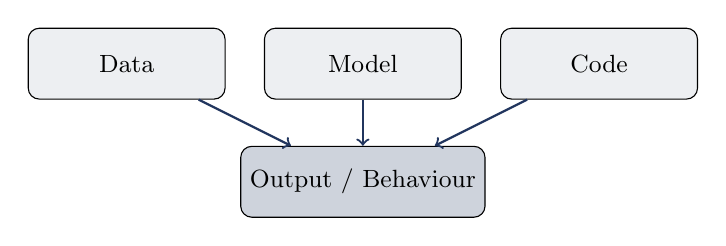
\begin{tikzpicture}[node distance=2cm, every node/.style={draw,rounded corners,fill=navy!8,minimum width=2.5cm,minimum height=0.9cm,align=center,font=\small}]
  \node (data) {Data};
  \node (model) [right of=data, xshift=1cm] {Model};
  \node (code) [right of=model, xshift=1cm] {Code};
  \node (output) [below of=model, yshift=0.5cm, fill=navy!22] {Output / Behaviour};
  \draw[->,thick,navy] (data) -- (output);
  \draw[->,thick,navy] (model) -- (output);
  \draw[->,thick,navy] (code) -- (output);
\end{tikzpicture}
\end{center}

Change the data (add more examples or remove biased ones) and the behaviour changes. Change the model architecture (switch from logistic regression to a neural network) and the behaviour changes. Change the code (bug in the preprocessing pipeline) and the behaviour changes. This three-way dependency makes debugging ML systems much harder than debugging traditional software.

\begin{watchout}
Do not test an ML system by only testing the code. A bug in the training data (mislabelled examples, wrong units) will silently produce wrong predictions even when all the code is correct. You must test data quality, model behaviour, and code together.
\end{watchout}

\subsection{The Model Lifecycle}

A \vocab{model} is a trained algorithm that accepts inputs and produces predictions or decisions. A model is not static — it has its own lifecycle:

\begin{enumerate}
  \item \textbf{Development} — choose an algorithm, train it on labelled data, tune hyperparameters.
  \item \textbf{Evaluation} — measure accuracy, precision, recall, AUC on a held-out test set.
  \item \textbf{Versioning} — save the trained model file and all metadata (training date, dataset version, metrics).
  \item \textbf{Deployment} — serve the model via an API so applications can call it.
  \item \textbf{Monitoring} — track prediction quality in production; detect data drift and performance degradation.
  \item \textbf{Retraining} — retrain on fresh data when performance drops below an acceptable threshold.
\end{enumerate}

\noindent\textbf{Where this shows up in ML/AI.} Every MLOps tool (MLflow, SageMaker, Vertex AI) is built around this lifecycle. When you hear ``ML pipeline'' in industry, this is what people mean.

%==============================================================
\section{The ML Pipeline}
%==============================================================

The \vocab{ML pipeline} is the end-to-end sequence of steps that takes raw data and produces a deployed, monitored model. It has two linked loops.

\subsection{The Static (Training) Pipeline}

\begin{center}
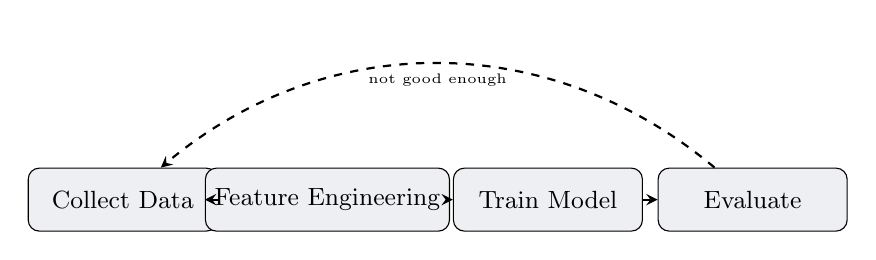
\begin{tikzpicture}[node distance=1.8cm,auto,>=stealth,font=\small,
  box/.style={draw,rounded corners,fill=navy!8,minimum width=2.4cm,minimum height=0.8cm,align=center}]
  \node[box] (collect) {Collect Data};
  \node[box, right of=collect, xshift=0.8cm] (features) {Feature Engineering};
  \node[box, right of=features, xshift=1cm] (train) {Train Model};
  \node[box, right of=train, xshift=0.8cm] (eval) {Evaluate};
  \draw[->,thick] (collect)--(features);
  \draw[->,thick] (features)--(train);
  \draw[->,thick] (train)--(eval);
  \draw[->,thick,dashed,bend right=40] (eval) to node[below,font=\tiny]{not good enough} (collect);
\end{tikzpicture}
\end{center}

\subsection{The Production Pipeline}

After the model passes evaluation, it enters production:

\begin{center}
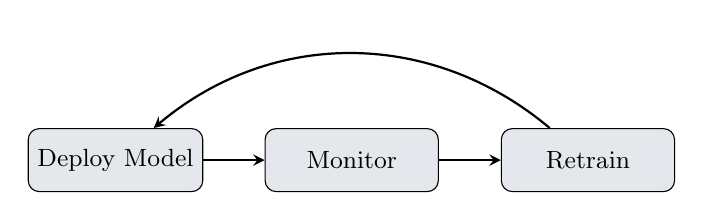
\begin{tikzpicture}[node distance=2.2cm,auto,>=stealth,font=\small,
  box/.style={draw,rounded corners,fill=navy!12,minimum width=2.2cm,minimum height=0.8cm,align=center}]
  \node[box] (deploy) {Deploy Model};
  \node[box, right of=deploy, xshift=0.8cm] (monitor) {Monitor};
  \node[box, right of=monitor, xshift=0.8cm] (retrain) {Retrain};
  \draw[->,thick] (deploy)--(monitor);
  \draw[->,thick] (monitor)--(retrain);
  \draw[->,thick,bend right=40] (retrain) to (deploy);
\end{tikzpicture}
\end{center}

\begin{worked}{Building a spam filter end to end}
We build a spam filter using the full ML pipeline. Start with 100{,}000 labelled emails.
\begin{steps}
  \item \textbf{Collect.} Gather 100{,}000 emails each labelled ``spam'' or ``not spam''.
  \item \textbf{Features.} Extract word counts, sender domain reputation, and link count from each email.
  \item \textbf{Train.} Fit a logistic regression model on 80{,}000 training emails.
  \item \textbf{Evaluate.} Test on 20{,}000 held-out emails. Result: precision 94\,\%, recall 91\,\%.
  \item \textbf{Deploy.} Expose the model as a REST API. Email servers call it for each incoming message.
  \item \textbf{Monitor.} Track how often users manually move emails to or from spam. If this rises above 10\,\%, the model is drifting.
  \item \textbf{Retrain.} Re-run the pipeline on the latest 30 days of emails every week.
\end{steps}
The pipeline is a cycle, not a one-time job. The model stays accurate because it keeps retraining on fresh data.
\end{worked}

%==============================================================
\section{Three Generations of Machine Learning}
%==============================================================

ML has evolved through three distinct generations, each solving problems the previous generation could not.

\begin{center}
\resizebox{\linewidth}{!}{%
\begin{tabular}{llll}
\toprule
\textbf{Generation} & \textbf{Era} & \textbf{Key technique} & \textbf{What you need} \\
\midrule
Gen 1: Classic ML & 1990s--2010s & Decision trees, SVMs, linear models & Labelled datasets, feature engineering \\
Gen 2: Deep Learning & 2012--2020 & Neural networks (CNN, RNN, LSTM) & Big data, GPU compute, labelled data \\
Gen 3: Transfer / Foundation & 2020--now & Pre-trained models, fine-tuning, APIs & A task description; no training required \\
\bottomrule
\end{tabular}}
\end{center}

\begin{everyday}
Gen 1 is like hiring an apprentice who learned only what you explicitly taught them. Gen 2 is like hiring a savant who read millions of books --- but you still had to supply the books. Gen 3 is like using a consultant who already knows everything. You tell them what you need and they deliver.
\end{everyday}

\begin{keytake}
Gen 3 (Foundation Models) lowers the bar to entry. A developer adds ML to an app by calling an API. No training data needed.
\end{keytake}

%==============================================================
\section{Types of ML Domains}
%==============================================================

ML is applied across many domains. The three most prevalent in industry are:

\subsection{Natural Language Processing (NLP)}

\vocab{NLP} teaches machines to understand, generate, and reason about human language. Human language is ambiguous, context-dependent, and culturally loaded --- making rule-based systems inadequate.

Examples: sentiment analysis, machine translation (Google Translate), document summarisation, question answering, chatbots.

\subsection{Computer Vision (CV)}

\vocab{Computer Vision} gives machines the ability to interpret images and video. Common uses: object detection (autonomous vehicles), face recognition (phone unlock), quality control (finding production-line defects), and medical imaging (detecting tumours).

\subsection{Speech Recognition}

\vocab{Automatic Speech Recognition (ASR)} converts spoken audio to text. Used in virtual assistants (Alexa, Siri, Google Assistant), transcription services, call-centre automation.

\noindent\textbf{Where this shows up in ML/AI.} Most modern ML apps combine domains. A voice assistant uses ASR (speech to text), then NLP (understand the question), then text-to-speech (answer). An autonomous car uses CV (see the road), NLP (process voice commands), and reinforcement learning (steer).

%==============================================================
\section{Foundation Models and Large Language Models}
%==============================================================

A \vocab{Foundation Model} is a large-scale model trained on a huge, broad dataset. Think: the entire web, all of Wikipedia, billions of images. After training it is adapted to specific tasks. Pre-training is expensive. Adaptation is cheap.

\begin{intuition}
Think of a foundation model as a university-educated generalist. They spent years learning widely (pre-training). You give them a two-week onboarding (fine-tuning) for your specific job. They are immediately productive. A Gen~1 specialist only knows what you explicitly taught them. They are only as good as the examples you gave them.
\end{intuition}

\vocab{Large Language Models (LLMs)} are the dominant type of foundation model today. They are trained on text. They can write, summarise, translate, answer questions, generate code, and reason step by step. Examples include GPT-4 (OpenAI), Claude 3.5 (Anthropic), Gemini (Google), LLaMA (Meta), DeepSeek, and Mistral.

\subsection{What an AI Engineer Needs to Know}

The modern \vocab{AI Engineer} role bridges software engineering and AI. Required skills:
\begin{itemize}
  \item Software engineering fundamentals: Python, SQL, Git, CI/CD, REST APIs.
  \item LLM integration: prompt engineering, RAG (Retrieval-Augmented Generation), fine-tuning.
  \item Model Context Protocol (MCP): connecting LLMs to external tools.
  \item MLOps: versioning, monitoring, deployment pipelines.
\end{itemize}

%==============================================================
\section{Software Engineering vs Machine Learning Engineering}
%==============================================================

SE and ML engineering are siblings, not twins. Knowing their differences is the first step to using SE skills in ML projects.

\begin{center}
\resizebox{\linewidth}{!}{%
\begin{tabular}{lll}
\toprule
\textbf{Dimension} & \textbf{Traditional SE} & \textbf{ML Engineering} \\
\midrule
Specification & Clear, explicit (requirements doc) & Fuzzy --- defined by data and metrics \\
Correctness & Deterministic: same input → same output & Probabilistic: output depends on model and data \\
Debugging & Trace code; add print statements & Inspect data; plot distributions; ablation studies \\
Testing & Unit tests with expected outputs & Test on held-out data; measure F1, AUC \\
Artefacts & Executable code & Executable code + trained model + dataset \\
Maintenance & Fix bugs, add features & Retrain; fix data pipelines; monitor drift \\
Failure mode & Exception thrown; stack trace & Silently wrong predictions \\
\bottomrule
\end{tabular}}
\end{center}

\housefig{figures/figsevml.png}{SE vs ML on four key dimensions. Blue bars show traditional SE; amber bars show ML engineering. Lower scores in ML mean harder and less predictable.}

\begin{watchout}
The most dangerous ML failure is a \emph{silent} one. A software bug crashes the program and announces itself. An ML model that starts giving wrong predictions may keep running for days before anyone notices. Monitoring is not optional.
\end{watchout}

\begin{worked}{SE rule vs ML model in a payment gateway}
A payment gateway uses fraud detection. Compare what happens when a rule breaks vs when a model breaks.
\begin{steps}
  \item \textbf{SE rule breaks.} The rule ``decline if country mismatches'' fires incorrectly. The team adds one exception and redeploys in a few hours. Done.
  \item \textbf{ML model breaks.} The model starts declining legitimate transactions from a new market. It was never trained on data from that market.
  \item \textbf{The symptom is invisible.} Customer complaints rise slowly. No stack trace. No crash. The model keeps running and serving wrong answers.
  \item \textbf{Fixing the ML model takes days.} Inspect model predictions on the new market. Check if the training set included that market. Retrain the model. Evaluate on a fresh test set. Then redeploy.
  \item \textbf{So what?} SE skills help you catch this early. Set up monitoring. Write tests for model behaviour. Version the training data.
\end{steps}
This is why adapting SE skills to ML is the whole point of this course.
\end{worked}

\begin{keytake}
ML shifts the source of truth from code to data. That one fact changes how you specify, test, debug, and maintain a system.
\end{keytake}

%==============================================================
\section*{Glossary \& Symbols}
\addcontentsline{toc}{section}{Glossary \& Symbols}
%==============================================================

\noindent\textbf{Key terms.}
\begin{description}[leftmargin=9em,style=nextline,font=\normalfont\bfseries\color{navy}]
  \item[SDLC] Software Development Life Cycle. A structured sequence of phases: plan, design, build, test, deploy, maintain.
  \item[Agile] A way of working in short sprints (1--3 weeks). Teams deliver working software continuously.
  \item[DevOps] A practice where development and operations share responsibility. Testing and deployment are automated.
  \item[Cloud Native] Building systems using containers, microservices, and cloud infrastructure. Systems are small and independent.
  \item[Data Science] The study of data: collecting it, cleaning it, analysing it, and drawing useful insights from it.
  \item[Machine Learning] A branch of AI where a program learns from data instead of being hand-programmed with rules.
  \item[ML Pipeline] The end-to-end sequence from raw data to a deployed, monitored model.
  \item[Model] A trained algorithm that takes inputs and produces predictions or decisions.
  \item[Data Drift] A change in the distribution of real-world data that makes an old model less accurate.
  \item[Foundation Model] A large model pre-trained on broad data, then adapted to specific tasks.
  \item[LLM] Large Language Model. A foundation model trained on text; can write, summarise, translate, and answer questions.
  \item[Fine-tuning] Extra training on task-specific data to adapt a foundation model.
  \item[RAG] Retrieval-Augmented Generation. A method that gives an LLM access to a document store at query time.
  \item[MLOps] Practices and tools for versioning, deploying, monitoring, and retraining ML models in production.
  \item[NLP] Natural Language Processing. Teaching machines to understand and generate human language.
  \item[ASR] Automatic Speech Recognition. Converts spoken audio to text.
  \item[CV] Computer Vision. Gives machines the ability to interpret images and video.
\end{description}

\medskip
\noindent\textbf{Abbreviations at a glance.}
\begin{center}\small
\begin{tabular}{@{}ll@{}}
\toprule
\textbf{Abbreviation} & \textbf{Stands for} \\
\midrule
SDLC & Software Development Life Cycle \\
ML & Machine Learning \\
AI & Artificial Intelligence \\
LLM & Large Language Model \\
NLP & Natural Language Processing \\
ASR & Automatic Speech Recognition \\
CV & Computer Vision \\
RAG & Retrieval-Augmented Generation \\
MLOps & Machine Learning Operations \\
MCP & Model Context Protocol \\
CI/CD & Continuous Integration / Continuous Deployment \\
AUC & Area Under the ROC Curve (a model quality measure) \\
\bottomrule
\end{tabular}
\end{center}

\end{document}
